\documentclass{beamer}
\usepackage[utf8x]{inputenc}
\usepackage{ucs}
\usepackage{amsmath}
\usepackage{amsfonts}
\usepackage{amssymb}
\usepackage{tikz}
\usetikzlibrary{arrows}
\usepackage{listings}
\usetheme{CambridgeUS}

\author{Cédric Guillot}
\institute{CPSC 565}
\title{Chess AI improvement through an evolutionary approach}
\date{April 9, 2013}

\begin{document}

\begin{frame}
\titlepage
\end{frame}

\begin{frame}
\begin{center}
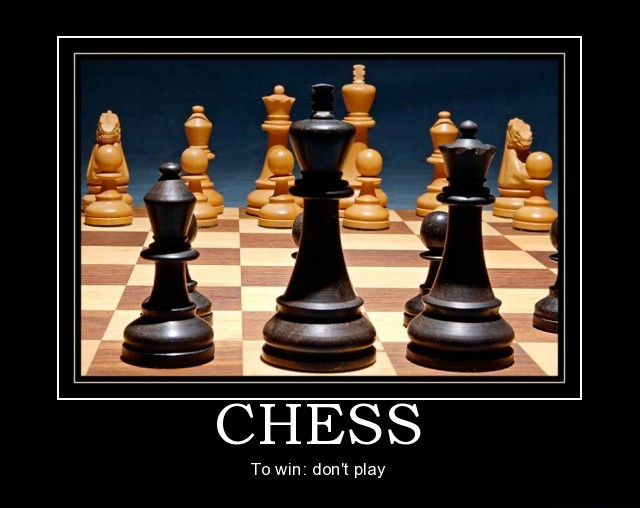
\includegraphics[scale=0.47]{images/to_win_dont_play.jpg}
\end{center}
\end{frame}

\begin{frame}
\tableofcontents
\end{frame}

\begin{frame}
\section{Introduction}
\subsection{???????}
\end{frame}

\begin{frame}
\section{Implementation / Strategy}
\subsection{Tools}
\frametitle{Tom Kerrigan's Simple Chess Program (TSCP)}
\begin{itemize}
\item Chess engine used for playing all the games
\item Written in 1997
\item Negamax algorithm for the AI
\end{itemize}
\end{frame}

\begin{frame}
\frametitle{GUI: GNU Xboard}
\begin{center}
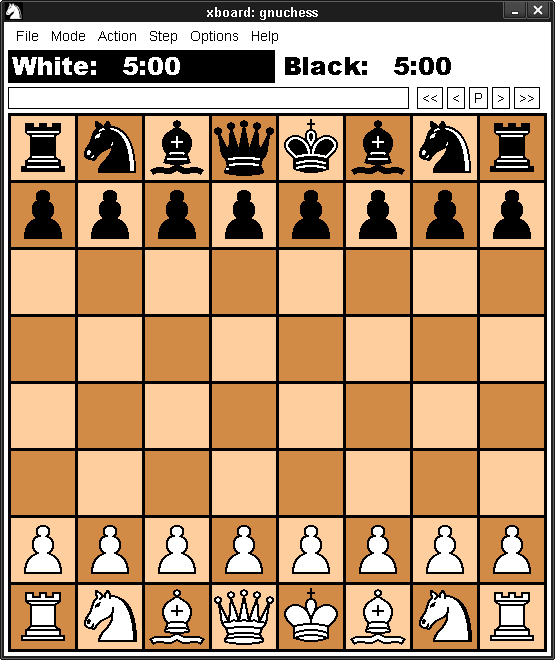
\includegraphics[scale=0.3]{images/xboard_view.png}
\end{center}
\end{frame}

\begin{frame}
\subsection{Architecture}
\frametitle{Architecture}
\begin{center}
\begin{figure}
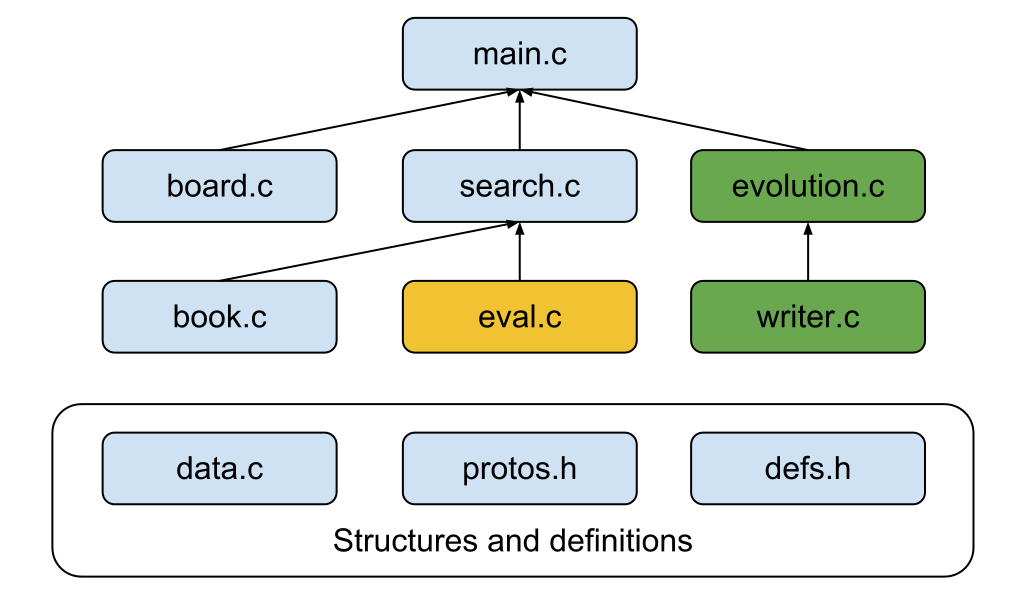
\includegraphics[scale=0.3]{images/Chess_AI_Architecture.png}
\caption{TSCP and evolution algorithm plugin architecture}
\end{figure}
\end{center}
\end{frame}

\begin{frame}
\subsection{Board evaluation / parameters evaluation}

\subsubsection{Rating system}
\subsection{•}
\end{frame}



\begin{frame}
\end{frame}

\begin{frame}
\end{frame}

\begin{frame}
\end{frame}

\begin{frame}

\end{frame}

\begin{frame}
\section{Results}
\subsection{Set-up}
\frametitle{Set-up}
\begin{itemize}
\item Search depth: n = 1
\item One day and a half running on a standard laptop
\item Optimized parameters: pawn, knight, bishop, rook and queen values
\item Evolution strategy parameters: $\mu = \frac{1}{2} \lambda = 4$
\item Static strategy parameters: RAND(-15, 15)
\end{itemize}
\end{frame}

\begin{frame}
\subsection{Original AI against me}
\subsection{Evoluted AI against me}
\subsection{Original AI against evoluted AI}
\end{frame}

\begin{frame}
\section{Future work}
\frametitle{Future work}
\end{frame}

\begin{frame}
\frametitle{References}
\end{frame}

\begin{frame}
\frametitle{Questions}
\begin{center}
\begin{Huge}
Any questions or suggestions?
\end{Huge}
\end{center}
\end{frame}

\end{document}